\paragraph{}
Cuando cambian las condiciones en un circuito, sus variables eléctricas evolucionan hasta llegar a un estado de equilibrio. A esta evolución se la denomina \emph{régimen transitorio}. \cite{apunte_guia4}
\paragraph{}
En este trabajo se estudiaron los regímenes transitorios de un circuito RC, un circuito RL, y el de un circuito RLC. 
\paragraph{}
Un circuito RC consiste de un resistor y un capacitor conectados en serie como muestra la figura \ref{esq: RC}. Si se conecta una fuente de ondas cuadradas de muy baja frecuencia, se puede estudiar la respuesta transitoria del circuito a un cambio repentino de potencial.
\begin{figure}[H]
    \centering
    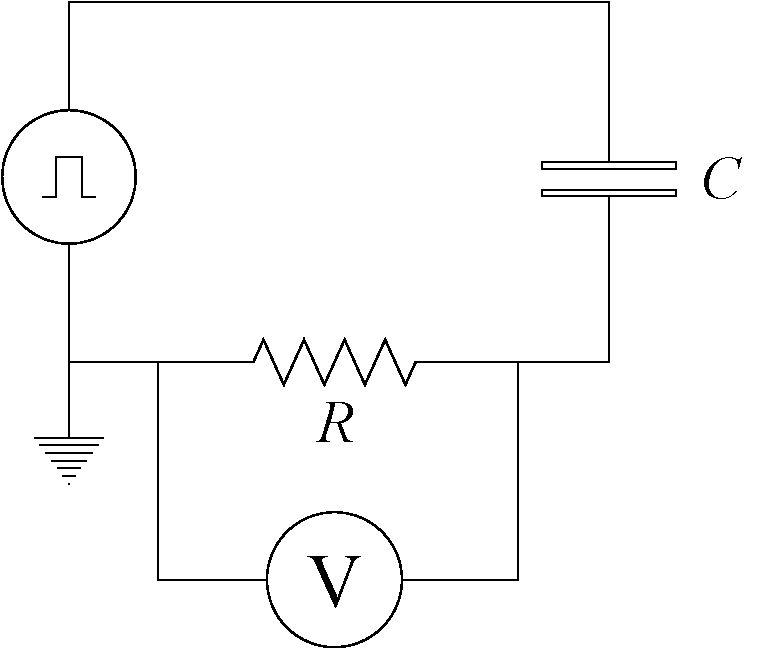
\includegraphics[scale= 0.45]{Esquemas/RC.drawio.pdf}
    \caption{Circuito RC, conformado por una fuente de ondas cuadradas, una capacitancia $C$ y una resistencia $R$ conectadas en serie. Se mide la caída de tensión en $R$ con un osciloscopio como voltímetro.}
    \label{esq: RC}
\end{figure}
\paragraph{}
La expresión para la caída de tensión a través del resistor para este circuito es \eqref{eqn:RC}
\begin{equation}\label{eqn:RC}
    V(t)=A\,e^{-t/\tau_{1}},
\end{equation}
siendo $A$ un coeficiente que depende de las condiciones iniciales del sistema y $\tau_{1}$ el tiempo característico del transitorio, dado por la ecuación \eqref{eqn:tau 1} \cite{apunte_guia4} 
\begin{equation}\label{eqn:tau 1}
    \tau_{1}=RC.
\end{equation}
\paragraph{}
Un circuito RL consiste un inductor y un resistor conectados en serie como muestra la figura \ref{esq: RL}.
\begin{figure}[H]
    \centering
    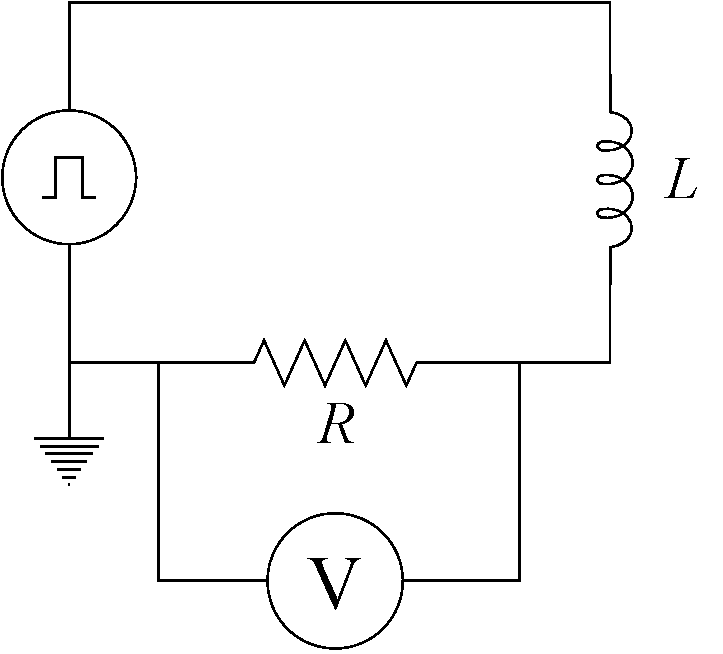
\includegraphics[scale= 0.5]{Esquemas/RL.drawio.pdf}
    \caption{Circuito RL alimentado por una fuente de ondas cuadradas y con una inductancia $L$ y una resistencia $R$ conectadas en serie. Al igual que en la figura \ref{esq: RL} se mide la caída de tensión en $R$ con un voltímetro}
    \label{esq: RL}
\end{figure}
La caída de tensión en el resistor $R$ está dada por la ecuación \eqref{eqn:RL}
\begin{equation}\label{eqn:RL}
    V(t)=A(1-e^{-t/\tau_2}),
\end{equation}
siendo $A$ un coeficiente que depende de las condiciones iniciales del sistema, y $\tau_2$ el tiempo característico del transitorio, dado por la expresión \eqref{eqn:tau 2} 
\begin{equation}\label{eqn:tau 2}
    \tau_2=\frac{L}{R}.
\end{equation}
\paragraph{}
Un circuito RLC esta conformado por un resistor, un capacitor y un inductor conectados en serie, como muestra la figura \ref{esq: RLC}.
\begin{figure}[H]
    \centering
    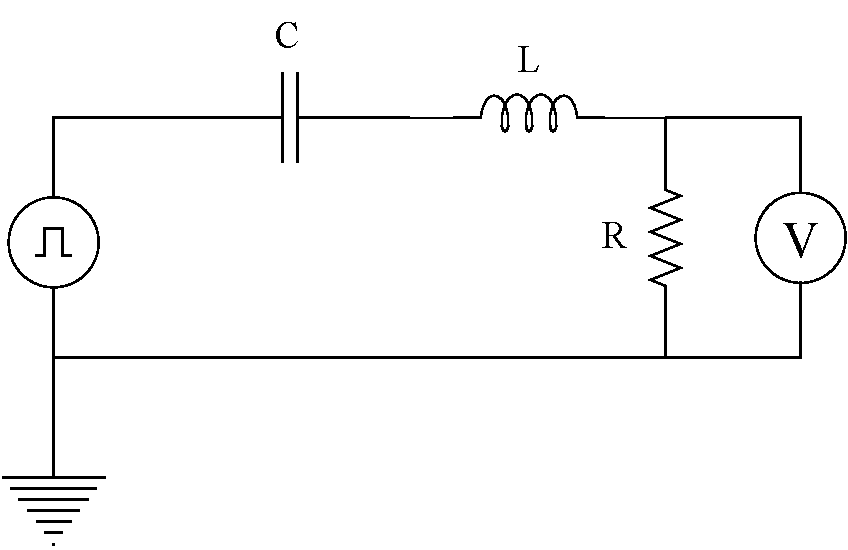
\includegraphics[scale= 0.5]{Esquemas/RLC.drawio.pdf}
    \caption{Esquema del circuito RLC, donde $R$ es la resistencia, $L$ es la inductancia y $C$ la capacitancia. Se utilizó un osciloscopio como voltímetro.}
    \label{esq: RLC}
\end{figure}
\paragraph{}
Las variables eléctricas de dicho circuito son análogas a las variables dinámicas de un oscilador armónico amortiguado, y al igual que este se pueden catalogar las respuestas para distintos valores de $R$, $L$ y $C$ en dos grupos dependiendo de si presentan una evolución oscilatoria o exponencial.
\paragraph{}
Se dice que el circuito presenta un régimen subamortiguado si se cumple la condición dada por \eqref{eqn:condicion sub}
\begin{equation}\label{eqn:condicion sub}
    R < 2\,\sqrt{\frac{L}{C}}.
\end{equation}
En este caso, la caída de tensión sobre el resistor viene dada por la ecuación \eqref{eqn:RLCsub}
\begin{equation}\label{eqn:RLCsub}
    V(t)=\frac{R \, V_0}{\omega \, L } \ e^{-\frac{R_{T}}{2L}t} \sin \left(\sqrt{\frac{1}{LC}-\left(\frac{R_{T}}{2L}\right)^2 }t\right).
\end{equation}
\paragraph{}
En cambio si se cumple la condición dada por \eqref{eqn:condicion sobre}
\begin{equation}\label{eqn:condicion sobre}
    R > 2\,\sqrt{\frac{L}{C}},
\end{equation}
se dice que el circuito presenta un régimen sobreamortiguado y la caída de tensión sobre el resistor viene dada por la ecuación \eqref{eqn:RLCsobre}
\begin{equation}\label{eqn:RLCsobre}
    V(t)=\frac{R \, V_0}{\sqrt{\left( \frac{R_{T}}{2}\right)^2-\frac{L}{C}}} \ e^{ -\frac{R_{T}}{2L}t} \sinh \left(\sqrt{\left(\frac{R_{T}}{2L}\right)^2-\frac{1}{LC}}\ t\right)
\end{equation}
\paragraph{}
En este trabajo se estudiaron los regímenes transitorios de circuitos RC, RL y RLC. En este último caso, se analizaron los casos subamortiguado y sobreamortiguado.